% ============================================================
% Oil Price Shocks and India's Terms of Trade
% An Empirical Assessment — Beamer Presentation
% ============================================================
\documentclass[10pt,aspectratio=169]{beamer}

% ------ Theme matching the reference image (dark blue header bar) ------
\usetheme{Copenhagen}
\usecolortheme{whale}
\setbeamercolor{structure}{fg=blue!80!black}
\setbeamercolor{frametitle}{bg=blue!75!black,fg=white}
\setbeamercolor{title}{bg=blue!75!black,fg=white}
\setbeamertemplate{navigation symbols}{}
\setbeamertemplate{footline}{%
  \hfill\insertframenumber/\inserttotalframenumber\hspace*{4pt}\vskip4pt}

% ------ Packages ------
\usepackage{graphicx}
\usepackage{booktabs}
\usepackage{amsmath,amssymb}
\usepackage{caption}
\usepackage{hyperref}
\usepackage{multirow}
\usepackage{array}
\usepackage[T1]{fontenc}

% ------ Graphics path ------
\graphicspath{{output/figures/}}

% ------ Title information ------
\title[Oil Price Shocks \& India's ToT]{Oil Price Shocks and India's Terms of Trade:\\An Empirical Assessment}
\subtitle{International Economics --- Group Presentation}
\author{Rehan Ansari \and Group Members}
\institute{Summer 2026}
\date{\today}

% ============================================================
\begin{document}

% ============================================================
% SLIDE 1 — Title
% ============================================================
\begin{frame}
  \titlepage
\end{frame}

% ============================================================
% SLIDE 2 — Outline
% ============================================================
\begin{frame}{Outline}
  \tableofcontents
\end{frame}

% ============================================================
\section{Introduction and Motivation}
% ============================================================

% SLIDE 3
\begin{frame}{Why Oil Prices and India's Terms of Trade?}
  \begin{itemize}
    \item India is the world's \textbf{3rd largest oil consumer}, importing $\sim$90\% of its crude.
    \item Simultaneously, India has developed a massive \textit{refined-petroleum export sector}.
    \item Every oil spike changes what India's exports can buy abroad.
    \vspace{0.3cm}
    \item \textbf{Key Indicator: Net Barter Terms of Trade (NTT)}
    \begin{equation*}
      NTT = \frac{\text{Export Unit Value Index}}{\text{Import Unit Value Index}} \times 100
    \end{equation*}
    \item A worsening ToT means India must give up more exports to purchase the same quantity of imports --- a real purchasing-power loss.
  \end{itemize}
\end{frame}

% SLIDE 4
\begin{frame}{Research Questions and Hypotheses}
  \begin{table}[ht]
    \centering\small
    \begin{tabular}{p{5.5cm} c p{7cm}}
      \toprule
      \textbf{Research Question} & \textbf{H} & \textbf{Main Conclusion} \\
      \midrule
      Do oil-price increases worsen India's ToT, and by how much? & H1 & \textbf{Supported.} Short-run elasticity $\approx -0.24$. \\[4pt]
      Do rises and falls have the same (symmetric) effect? & H2 & \textbf{Not supported.} Effects are broadly symmetric. \\[4pt]
      Does it matter whether oil became expensive because of a supply cut or a demand boom? & H3 & \textbf{Not supported.} Demand shocks hurt at least as much. \\[4pt]
      Has India's exposure changed over time? & Ext. & \textbf{Yes.} Exposure roughly halved since the 1990s. \\
      \bottomrule
    \end{tabular}
  \end{table}
\end{frame}

% ============================================================
\section{Historical Stylized Facts}
% ============================================================

% SLIDE 5
\begin{frame}{Oil Prices vs.\ India's Terms of Trade (1970--2025)}
  \begin{figure}
    \centering
    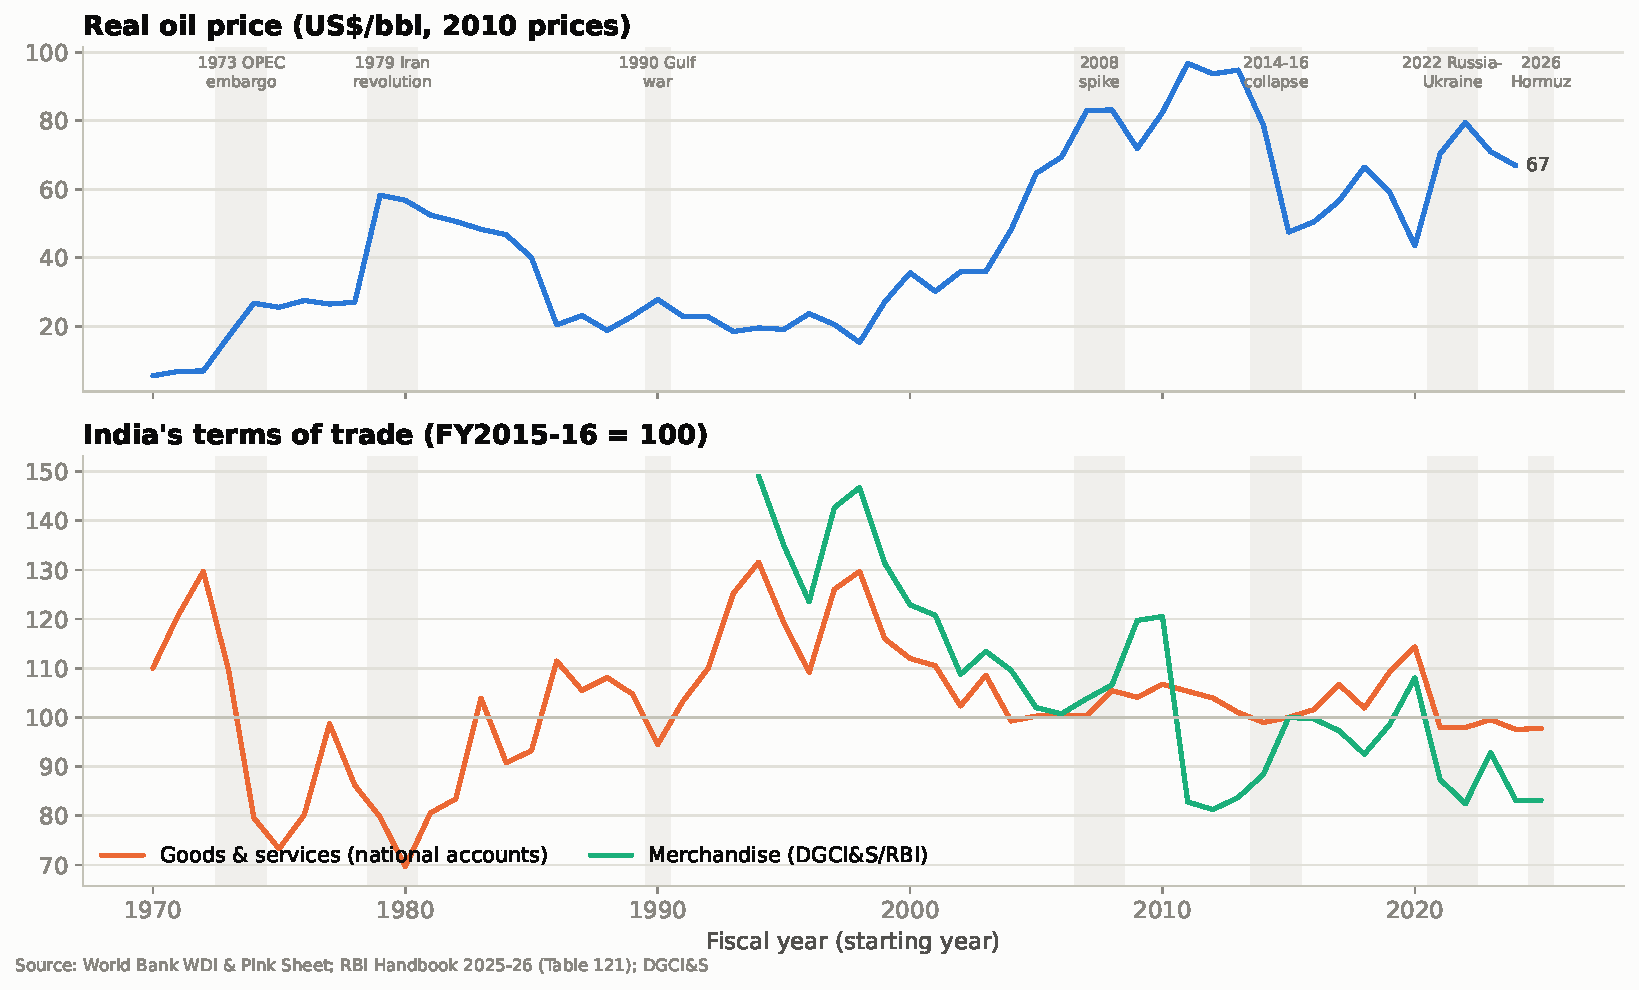
\includegraphics[height=0.68\textheight]{fig01_tot_vs_real_oil_annual.pdf}
    \caption{Real Oil Price and India's Goods \& Services ToT, FY1970--71 to FY2025--26}
  \end{figure}
\end{frame}

% SLIDE 6
\begin{frame}{Major Oil-Price Episodes}
  \begin{table}[ht]
    \centering\small
    \begin{tabular}{l l r}
      \toprule
      \textbf{Episode} & \textbf{Period} & \textbf{G\&S ToT Change} \\
      \midrule
      OPEC Embargo & 1973--74 & $-38.6\%$ \\
      Iranian Revolution & 1979--80 & $-19.2\%$ \\
      Gulf War & 1990--91 & $-12.8\%$ \\
      2007--08 Commodity Boom & 2007--08 & $-8.9\%$ \\
      Russia-Ukraine & 2022--23 & $-23.7\%$ (merchandise) \\
      2026 Hormuz & 2025--26 & Data provisional \\
      \bottomrule
    \end{tabular}
    \caption{Major oil-price episodes and India's ToT response}
  \end{table}
  \begin{itemize}
    \item Major oil-price increases consistently coincide with ToT deterioration.
    \item The 2022 Russia-Ukraine shock saw merchandise ToT collapse by $\sim$23.7\%.
  \end{itemize}
\end{frame}

% SLIDE 7
\begin{frame}{Monthly Merchandise ToT and Brent Crude}
  \begin{figure}
    \centering
    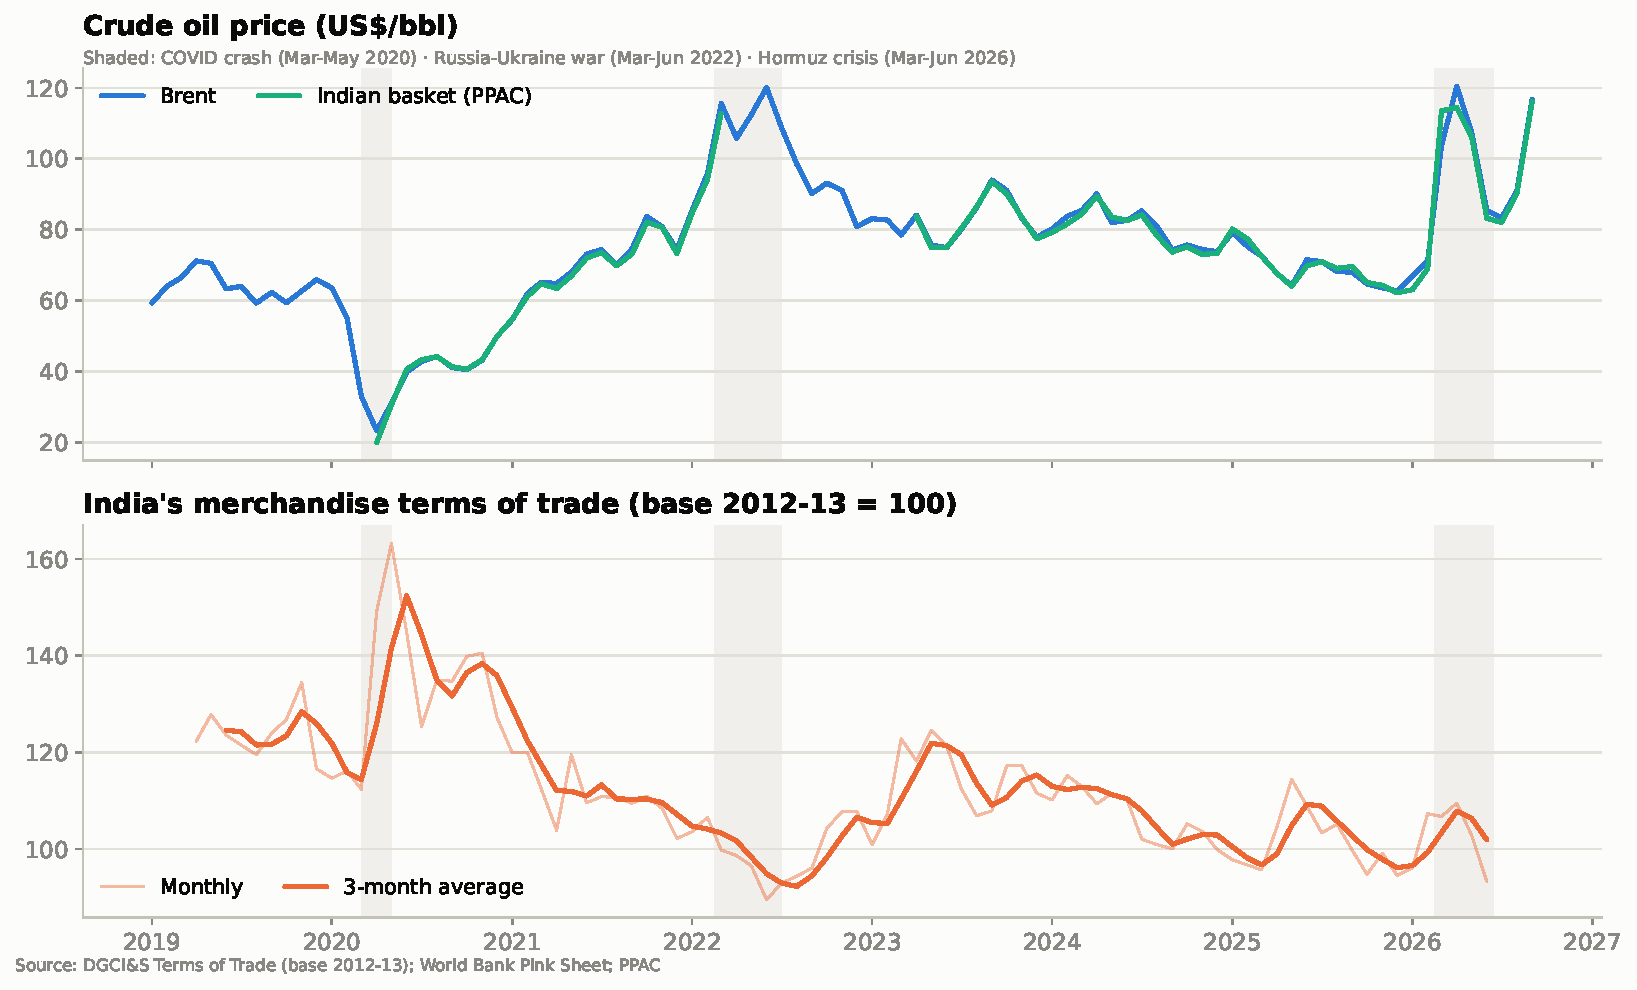
\includegraphics[height=0.68\textheight]{fig02_monthly_ntt_brent.pdf}
    \caption{Monthly Merchandise NTT and Brent Crude Price (Apr 2019--Jun 2026)}
  \end{figure}
\end{frame}

% ============================================================
\section{Theoretical Framework}
% ============================================================

% SLIDE 8
\begin{frame}{Offer Curves: How Oil Shocks Transmit}
  \begin{figure}
    \centering
    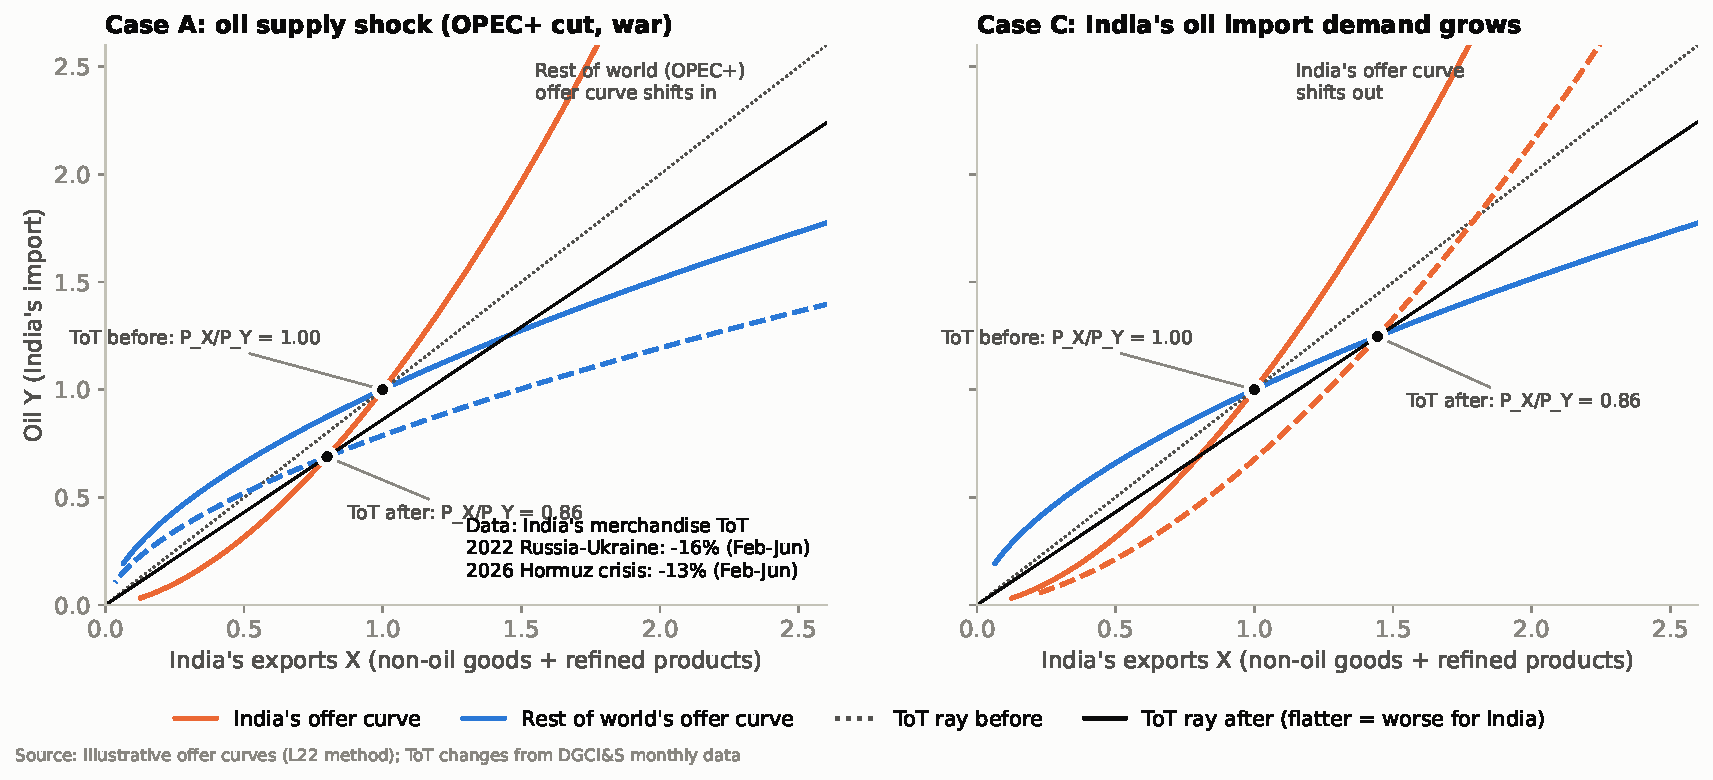
\includegraphics[height=0.55\textheight]{fig07_offer_curves_india.pdf}
    \caption{Offer Curves: Supply Cut (Left Panel) and India Demand Expansion (Right Panel)}
  \end{figure}
  \begin{itemize}
    \item \textbf{Supply Disruption:} Oil exporters offer less at each trade ratio $\Rightarrow$ ToT ray rotates inward (worsens for India).
    \item \textbf{India Demand Expansion:} India is not a pure price-taker (5.4\% of world consumption). Its own demand pushes against inelastic world supply.
  \end{itemize}
\end{frame}

% SLIDE 9
\begin{frame}{Theory Benchmark: How Big Should the Hit Be?}
  \begin{columns}[T]
    \begin{column}{0.5\textwidth}
      \begin{figure}
        \centering
        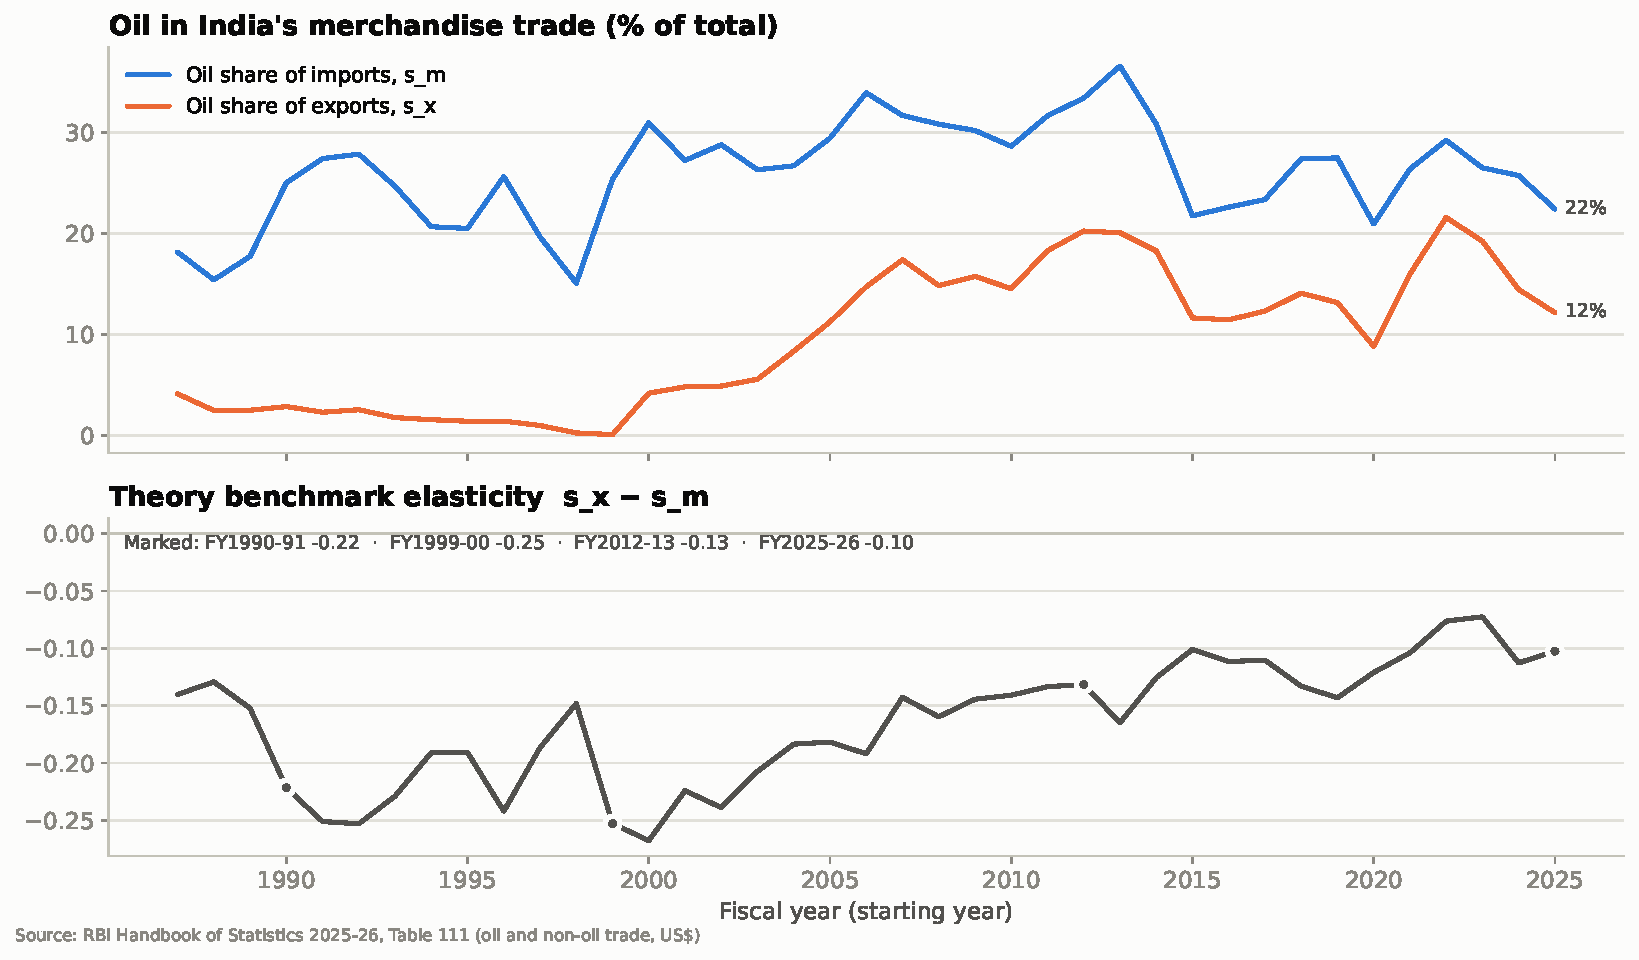
\includegraphics[height=0.55\textheight]{fig03_oil_shares_benchmark.pdf}
        \caption{Oil's share in merchandise imports ($s_m$) and exports ($s_x$)}
      \end{figure}
    \end{column}
    \begin{column}{0.5\textwidth}
      \textbf{Benchmark Formula:}
      \begin{equation*}
        d \ln(NTT) \approx (s_x - s_m)\, d \ln(P_{\text{oil}})
      \end{equation*}
      \begin{itemize}
        \item Since $s_m > s_x$, the coefficient is \textbf{negative}: oil-price rises worsen ToT.
        \item As India's refined petroleum exports grow ($s_x$ rises), the net gap $(s_m - s_x)$ \textbf{shrinks}.
        \item Theory benchmark: $-0.25 \to -0.10$ over the sample.
      \end{itemize}
    \end{column}
  \end{columns}
\end{frame}

% SLIDE 10
\begin{frame}{India's Import Dependence: Volume vs.\ Bill}
  \begin{figure}
    \centering
    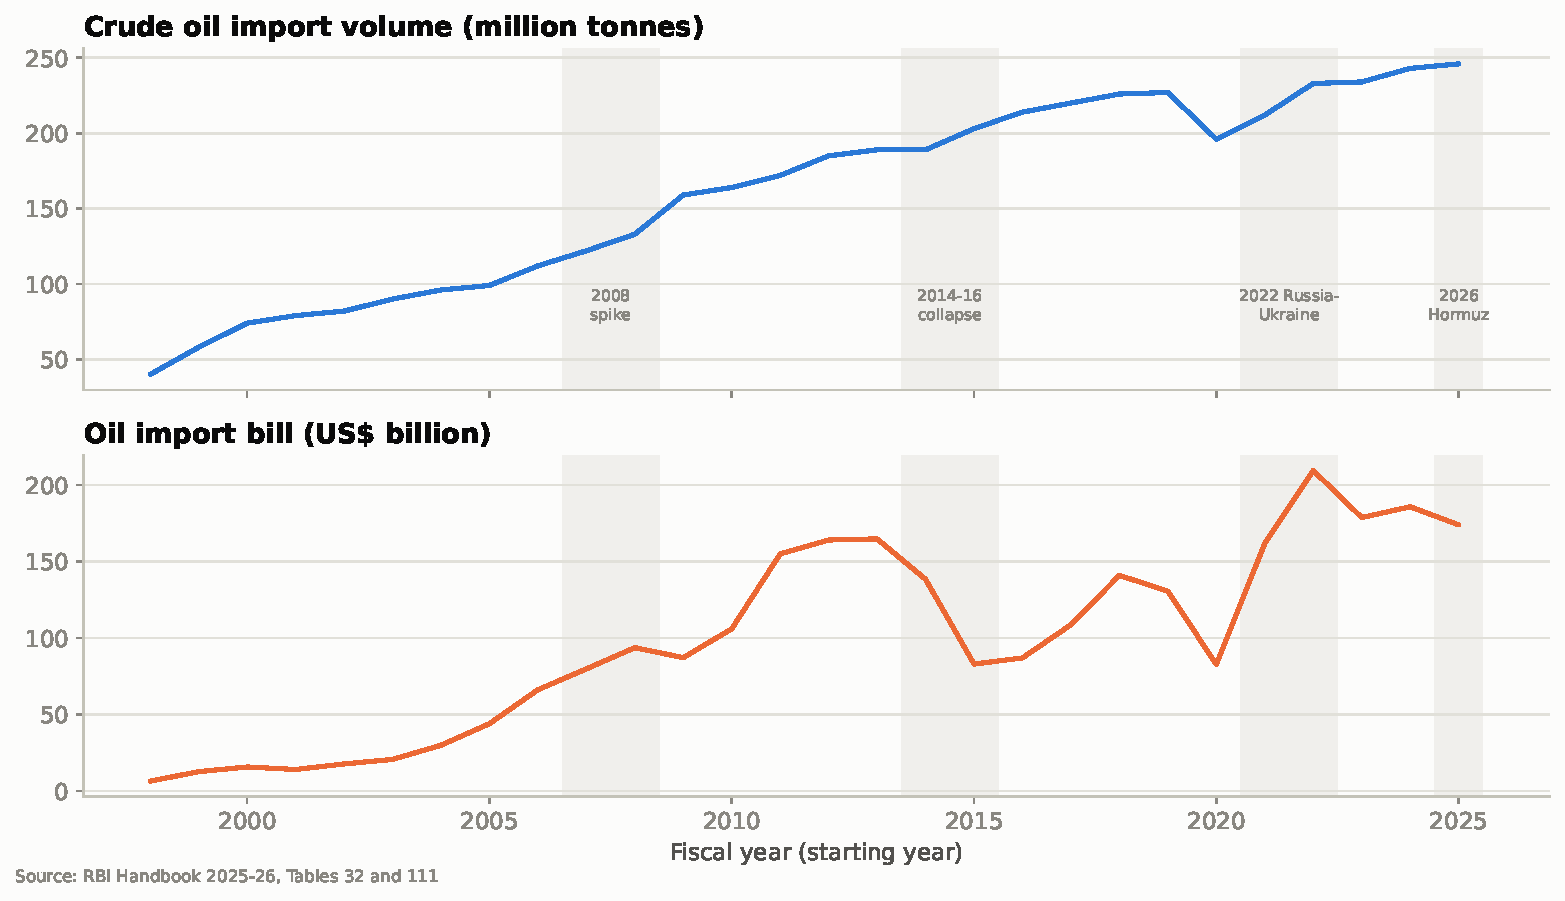
\includegraphics[height=0.68\textheight]{fig06_import_volume_vs_bill.pdf}
    \caption{Crude oil import volume vs.\ the oil import bill}
  \end{figure}
\end{frame}

% ============================================================
\section{Data}
% ============================================================

% SLIDE 11
\begin{frame}{Data Architecture and Quality}
  \begin{columns}[T]
    \begin{column}{0.5\textwidth}
      \textbf{Datasets:}
      \begin{itemize}
        \item \textit{Annual long run} (FY1970--2025): World Bank G\&S ToT deflators; RBI merchandise UVIs.
        \item \textit{Monthly} (Apr 2019--Jun 2026): DGCI\&S merchandise NTT (2019--20 episodes).
        \item \textit{Real oil price:} Brent deflated by WB Manufactured Unit Value (MUV) index.
      \end{itemize}
    \end{column}
    \begin{column}{0.5\textwidth}
      \textbf{Sources:}
      \begin{itemize}
        \item RBI, DGCI\&S, PPAC
        \item World Bank, UNCTAD, UN Comtrade
        \item EIA, BIS
        \item Baumeister--Hamilton (2019), K\"anzig (2021) shock series
      \end{itemize}
      \vspace{0.3cm}
      \textbf{Validation:}
      \begin{itemize}
        \item Overlap-ratio linking for base-year fixes.
        \item Cross-checked vs.\ UN Comtrade (0 failures).
      \end{itemize}
    \end{column}
  \end{columns}
\end{frame}

% ============================================================
\section{Methodology}
% ============================================================

% SLIDE 12
\begin{frame}{Empirical Strategy}
  \begin{enumerate}
    \item \textbf{H1 --- ARDL in Error-Correction Form:}
    \begin{equation*}
      \Delta \ln NTT_t = \alpha + \phi\, (NTT_{t-1} - \hat{\beta}\, \text{Oil}_{t-1}) + \gamma\, \Delta \ln \text{Oil}_t + \sum \delta_j \Delta \ln NTT_{t-j} + u_t
    \end{equation*}
    Separates short-run elasticity ($\gamma$) from the long-run relationship.

    \item \textbf{H2 --- NARDL Asymmetry:}\\
    Decomposes oil-price changes into cumulative increases ($\text{Oil}^+$) and decreases ($\text{Oil}^-$).

    \item \textbf{Timing --- Jord\`a Local Projections:}\\
    Estimates ToT response at direct monthly horizons $h = 0, 1, \ldots, 6$.

    \item \textbf{H3 --- Structural Shock Identification:}\\
    Baumeister--Hamilton (2019) decomposition for supply vs.\ demand.\\
    K\"anzig (2021) OPEC supply-news shocks as exogenous cross-check.
  \end{enumerate}
\end{frame}

% ============================================================
\section{Results}
% ============================================================

% SLIDE 13
\begin{frame}{H1: Oil Prices Worsen India's Terms of Trade}
  \begin{table}[ht]
    \centering\small
    \begin{tabular}{lcccl}
      \toprule
      \textbf{Parameter} & \textbf{Estimate} & \textbf{SE} & \textbf{p-value} & \textbf{Interpretation} \\
      \midrule
      Short-run elasticity ($\gamma$) & $-0.241$ & 0.040 & $<0.001$ & 10\% oil rise $\Rightarrow$ 2.4\% ToT fall \\[3pt]
      Long-run elasticity ($\hat{\beta}$) & $-0.092$ & 0.059 & 0.12 & Small, not significant \\[3pt]
      Error-correction ($\phi$) & $-0.308$ & 0.086 & 0.001 & 31\% gap corrected per year \\[3pt]
      Bounds F-stat & \multicolumn{2}{c}{4.74} & $>$ I(1) CV & Cointegration confirmed \\[3pt]
      $R^2$ / Adj.\ $R^2$ & \multicolumn{2}{c}{0.59 / 0.56} & & \\
      \bottomrule
    \end{tabular}
    \caption{ARDL(1,0) baseline results --- Annual G\&S ToT, FY1970--2025}
  \end{table}
  \textbf{Takeaway:} Sharp short-run deterioration followed by adjustment --- not a permanent hit.
\end{frame}

% SLIDE 14
\begin{frame}{Model Diagnostics and Stability}
  \begin{columns}[T]
    \begin{column}{0.5\textwidth}
      \begin{table}[ht]
        \centering\footnotesize
        \begin{tabular}{lcc}
          \toprule
          \textbf{Test} & \textbf{Statistic} & \textbf{p-value} \\
          \midrule
          Breusch--Godfrey & BG(1) & Pass \\
          ARCH-LM & $\chi^2$ & Pass \\
          Jarque--Bera & JB & Pass \\
          Ramsey RESET & F & Pass \\
          \bottomrule
        \end{tabular}
        \caption{Residual diagnostics}
      \end{table}
    \end{column}
    \begin{column}{0.5\textwidth}
      \begin{figure}
        \centering
        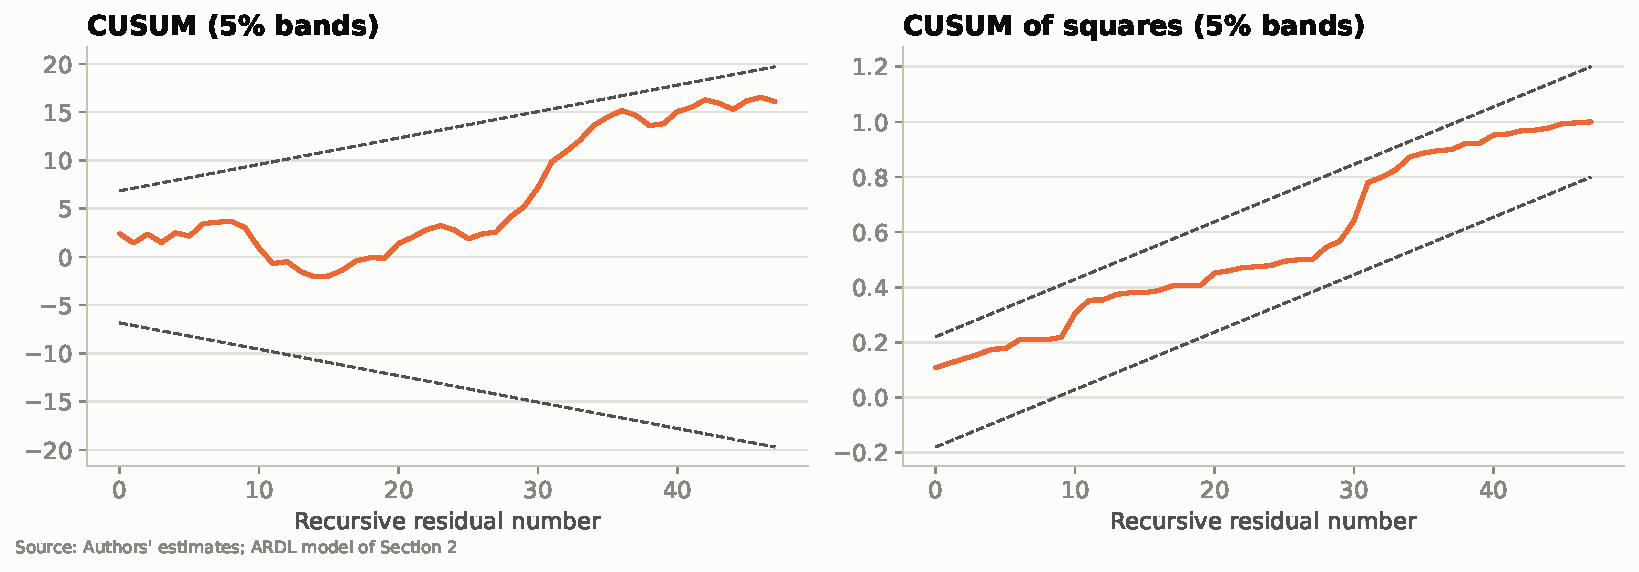
\includegraphics[height=0.55\textheight]{fig08_cusum_stability.pdf}
        \caption{CUSUM stability test --- parameters within 5\% bounds}
      \end{figure}
    \end{column}
  \end{columns}
\end{frame}

% SLIDE 15
\begin{frame}{Timing: When Does the Hit Arrive?}
  \begin{figure}
    \centering
    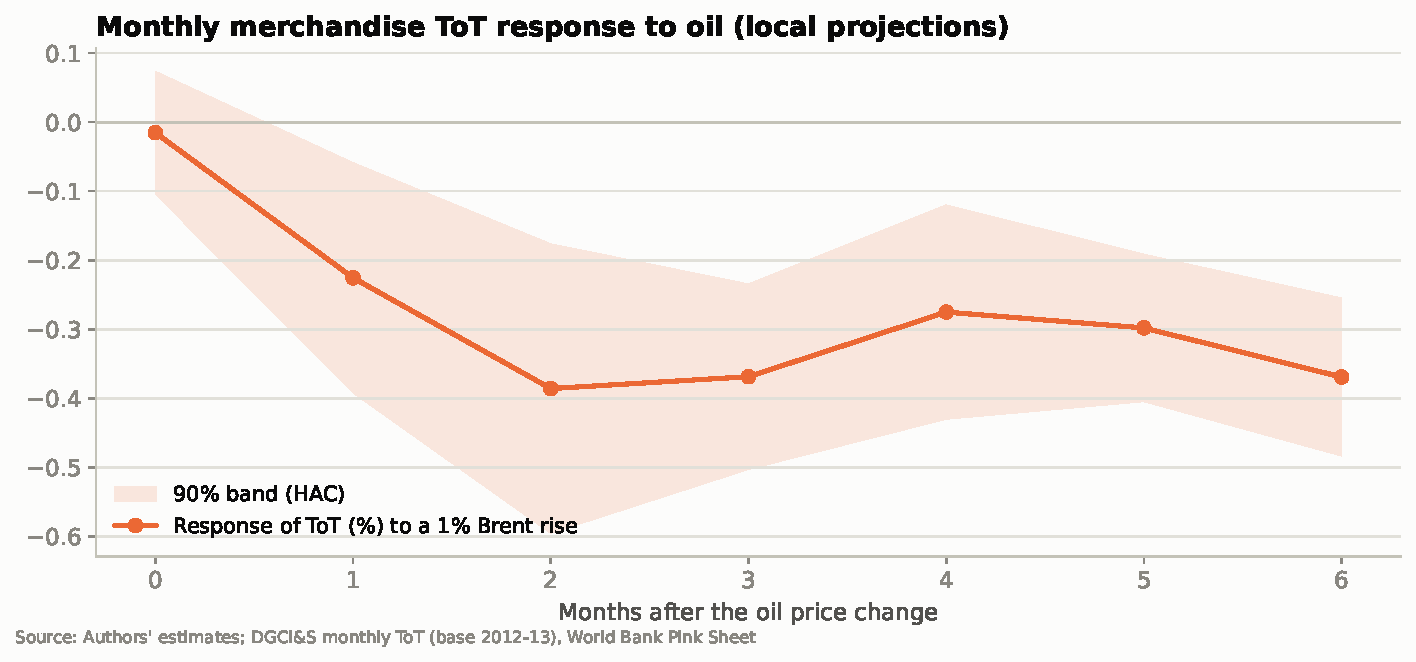
\includegraphics[height=0.6\textheight]{fig11_local_projections_monthly.pdf}
    \caption{Monthly Local Projections: ToT response at horizons $h = 0, \ldots, 6$ months}
  \end{figure}
  \begin{itemize}
    \item Contemporaneous effect $\approx -0.02$ (near zero).
    \item \textbf{Peak elasticity $\approx -0.39$ after two months.}
    \item Consistent with contract pricing lags, shipping times, and inventory adjustment.
  \end{itemize}
\end{frame}

% SLIDE 16
\begin{frame}{H2: Are Rises and Falls Asymmetric?}
  \begin{columns}[T]
    \begin{column}{0.55\textwidth}
      \begin{figure}
        \centering
        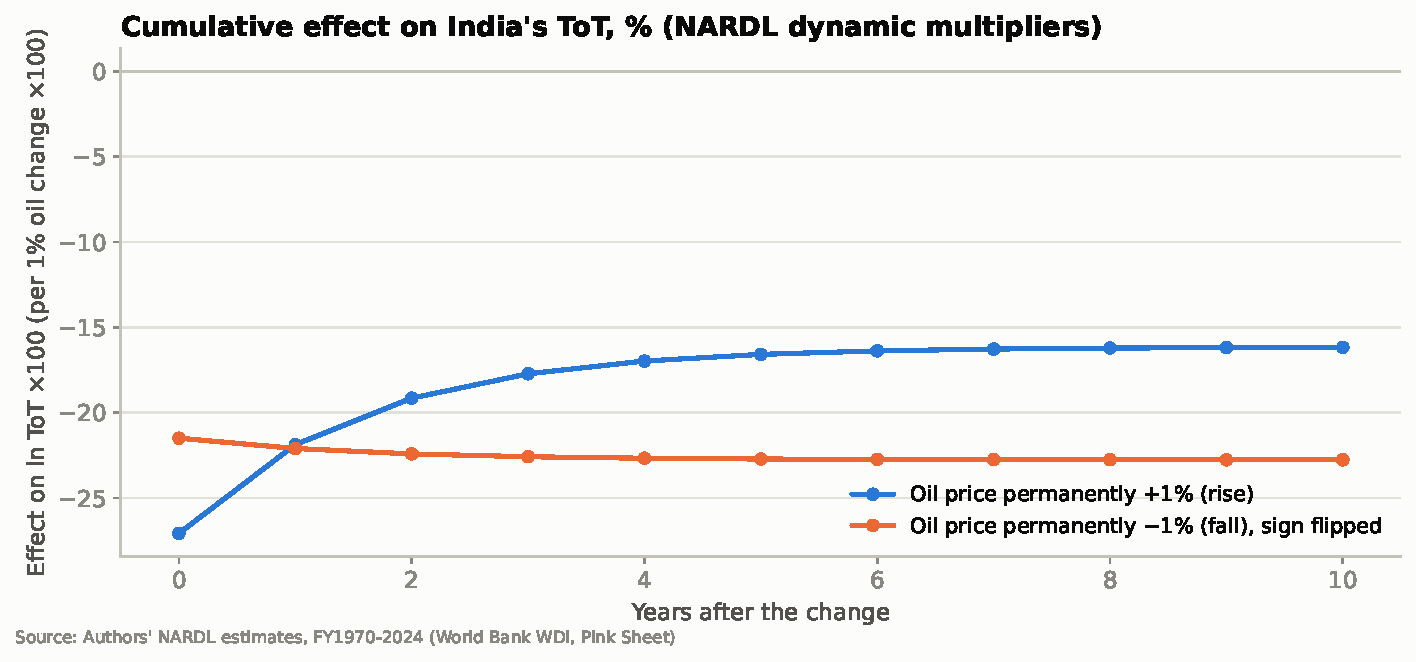
\includegraphics[height=0.55\textheight]{fig09_nardl_multipliers.pdf}
        \caption{NARDL dynamic multipliers: positive vs.\ negative shocks}
      \end{figure}
    \end{column}
    \begin{column}{0.45\textwidth}
      \textbf{Result: Not supported.}
      \begin{itemize}
        \item Short-run: $-0.27$ (rises) vs.\ $-0.22$ (falls)
        \item Wald test for symmetry: $p = 0.54$--$0.91$
        \item Asymmetry never rejected across specifications.
      \end{itemize}
      \vspace{0.3cm}
      \textbf{Implication:} Fiscal policy can smooth \textit{both} spikes and slumps symmetrically.
    \end{column}
  \end{columns}
\end{frame}

% SLIDE 17
\begin{frame}{Declining Exposure: Rolling Elasticity}
  \begin{figure}
    \centering
    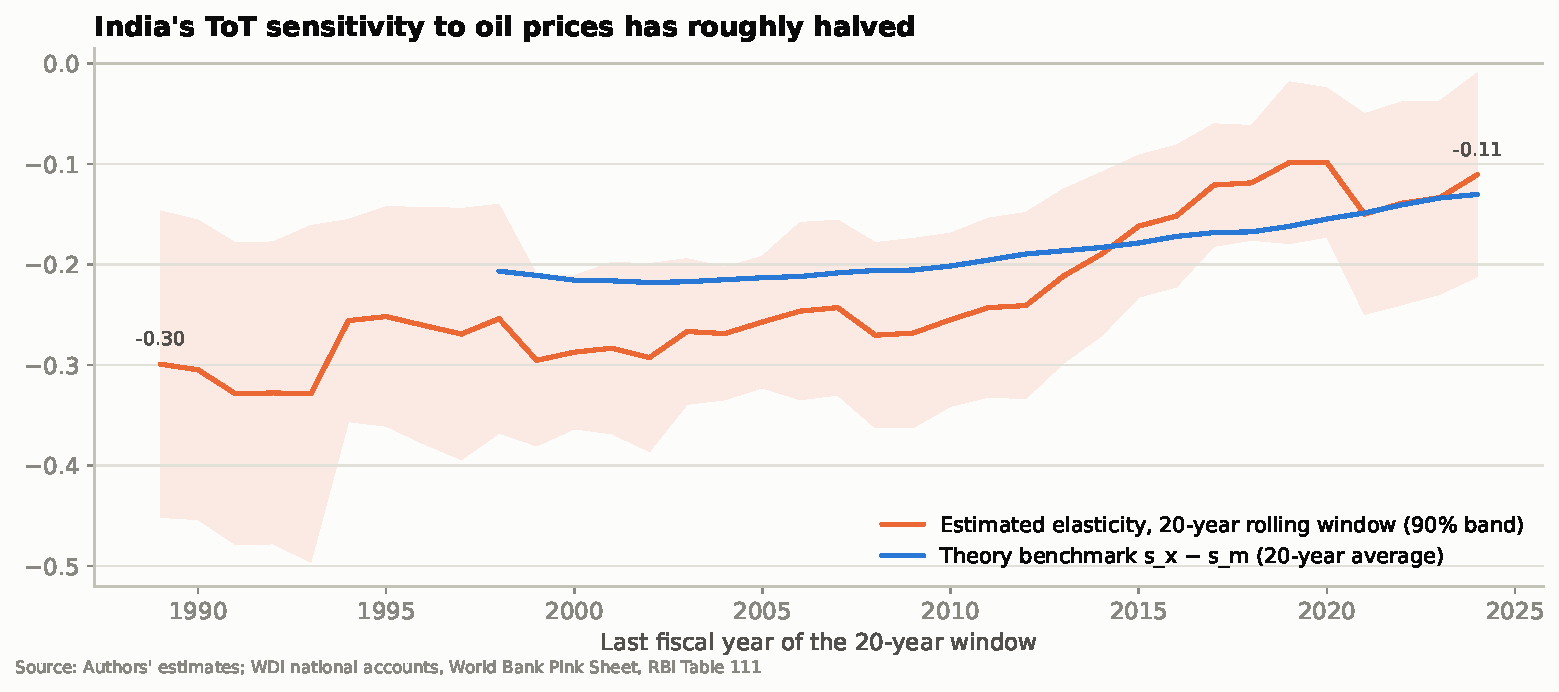
\includegraphics[height=0.6\textheight]{fig10_rolling_elasticity.pdf}
    \caption{Rolling 20-year short-run oil-price elasticity of India's ToT}
  \end{figure}
  \begin{itemize}
    \item Elasticity roughly halves: $\mathbf{-0.30 \to -0.11}$.
    \item Closely tracks theory benchmark decline ($-0.25 \to -0.10$).
  \end{itemize}
\end{frame}

% SLIDE 18
\begin{frame}{H3: Supply vs.\ Demand Shocks}
  \begin{columns}[T]
    \begin{column}{0.55\textwidth}
      \begin{figure}
        \centering
        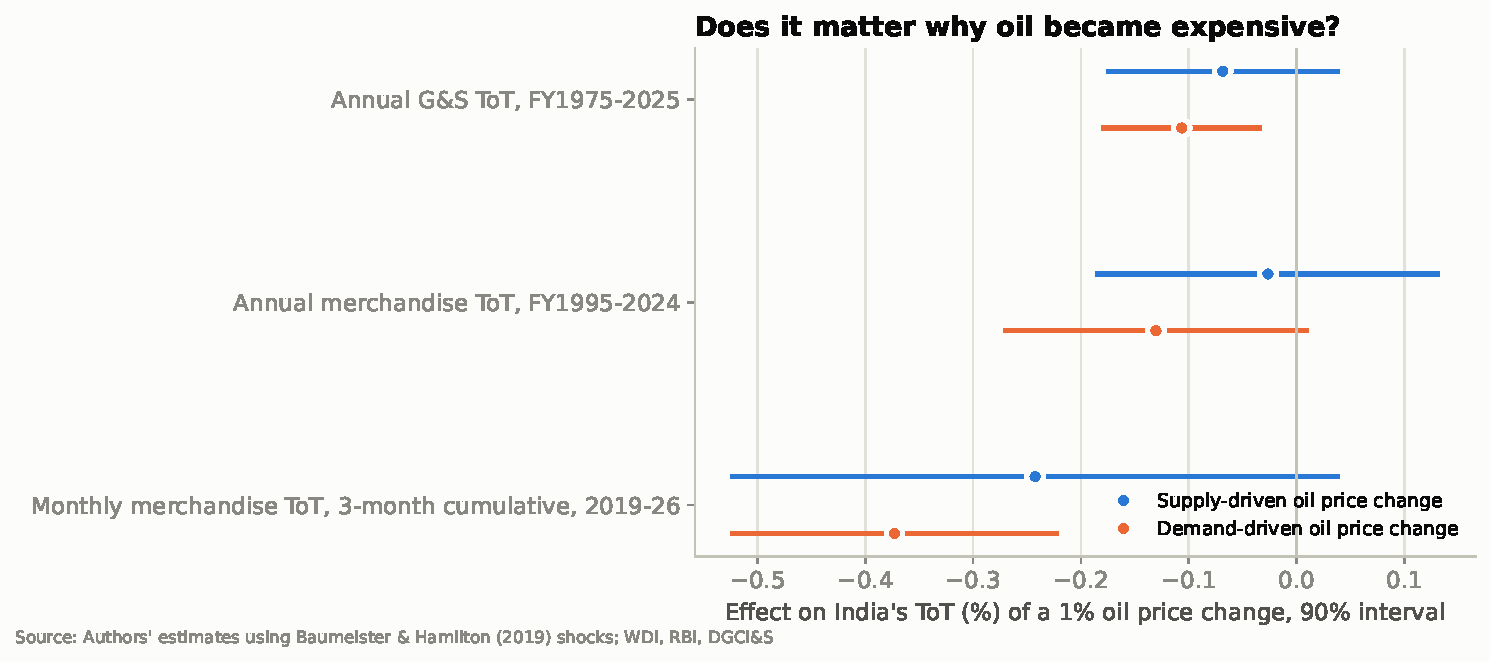
\includegraphics[height=0.55\textheight]{fig12_supply_vs_demand.pdf}
        \caption{Supply-driven vs.\ demand-driven effects on ToT}
      \end{figure}
    \end{column}
    \begin{column}{0.45\textwidth}
      \textbf{Result: Not supported.}
      \begin{itemize}
        \item Demand-driven rises hurt at least as much as supply-driven ones.
        \item Equality never rejected ($p = 0.53$--$0.71$).
        \item K\"anzig OPEC news shocks: $4$--$5\%$ ToT decline.
      \end{itemize}
      \vspace{0.3cm}
      \textbf{Why?} A global demand boom lifts prices of \textit{multiple} imported commodities (oil, coal, fertilizer, metals), offsetting any gains in export demand.
    \end{column}
  \end{columns}
\end{frame}

% ============================================================
\section{Structural Explanation: The Refining Hedge}
% ============================================================

% SLIDE 19
\begin{frame}{India's Acquired Comparative Advantage in Refining}
  \begin{figure}
    \centering
    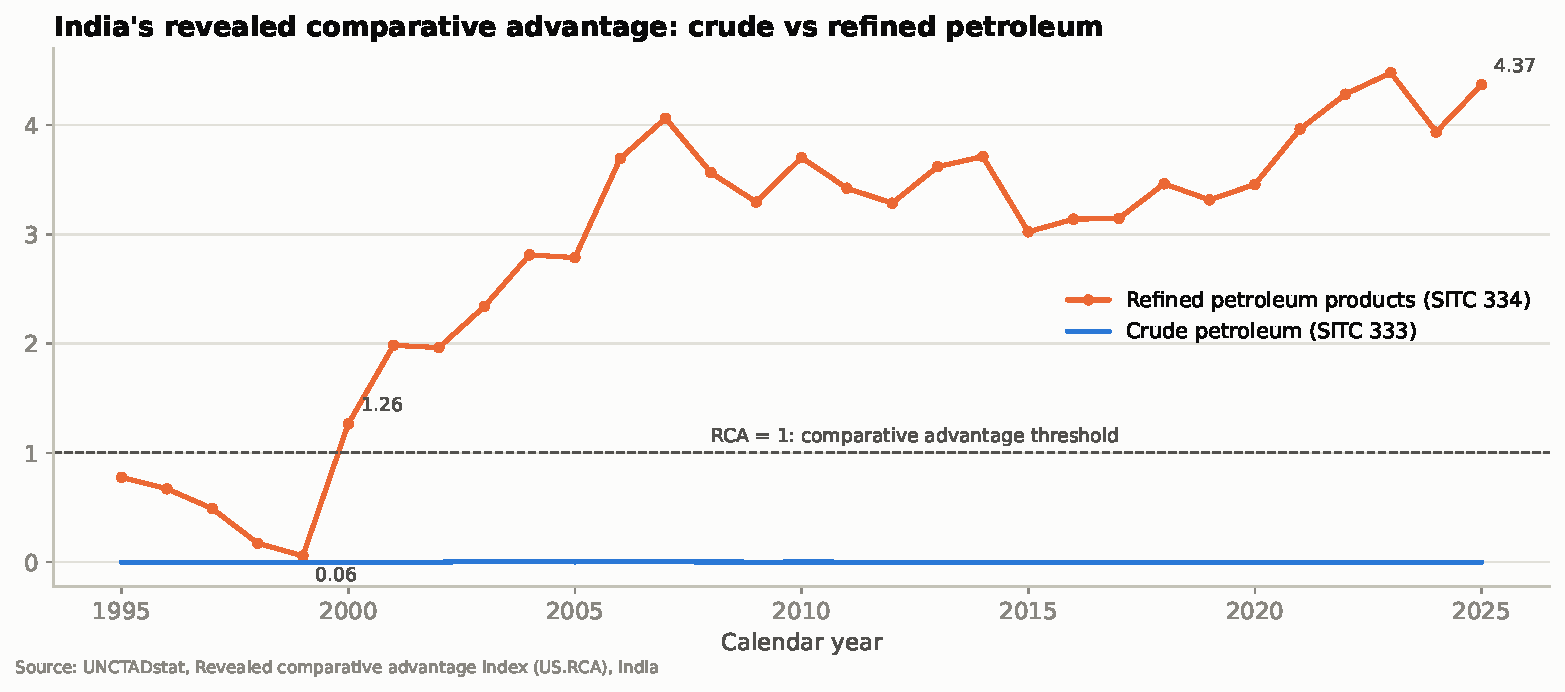
\includegraphics[height=0.6\textheight]{fig04_rca_refined_petroleum.pdf}
    \caption{Revealed Comparative Advantage (RCA) in Refined Petroleum (HS 2710)}
  \end{figure}
  \begin{itemize}
    \item RCA rose from \textbf{0.06} (1999) to \textbf{4.37} (2025) --- a 70$\times$ increase.
    \item India imports lower-value crude, exports higher-value refined products.
    \item Higher oil prices increase export values $\Rightarrow$ endogenous hedge.
  \end{itemize}
\end{frame}

% SLIDE 20
\begin{frame}{Vertical Processing Trade: Grubel--Lloyd Decomposition}
  \begin{figure}
    \centering
    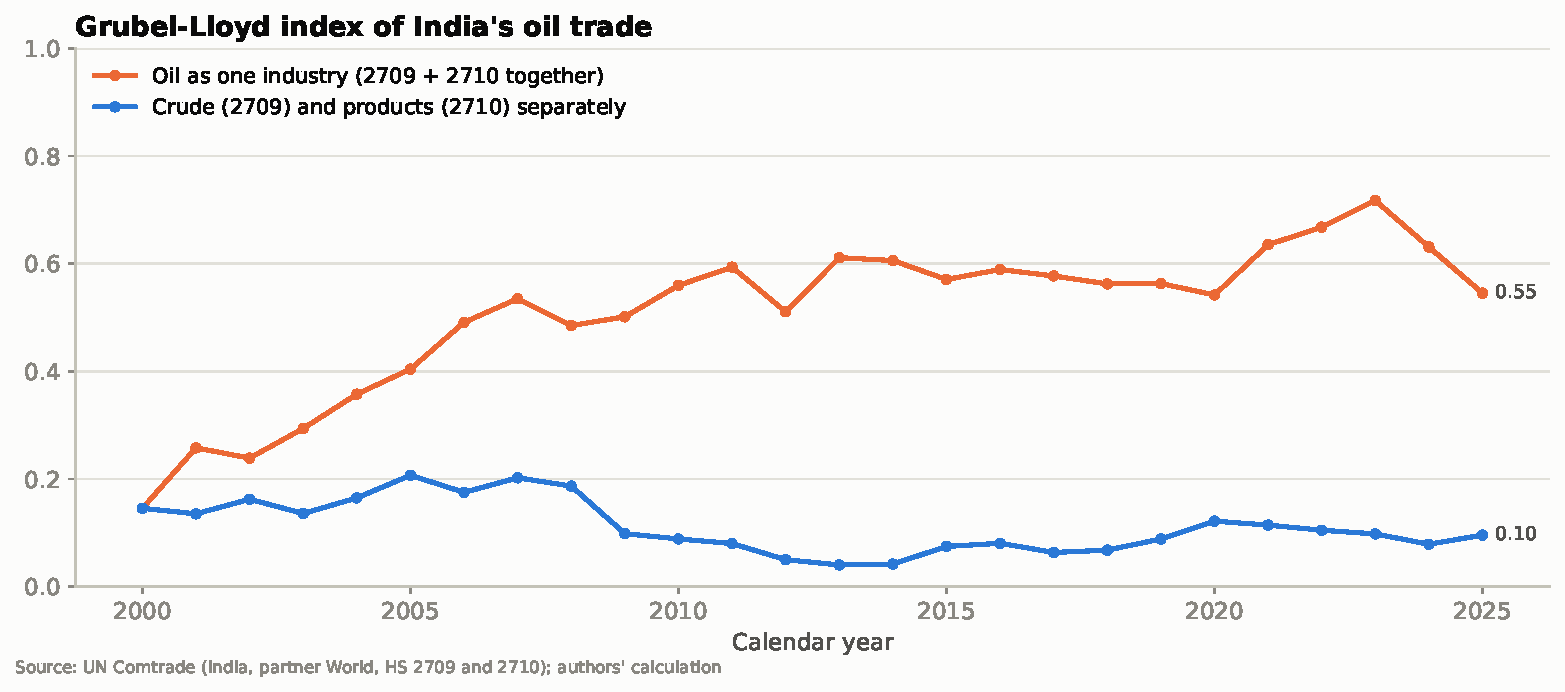
\includegraphics[height=0.6\textheight]{fig05_grubel_lloyd_aggregation.pdf}
    \caption{Grubel--Lloyd Index: aggregate vs.\ crude/refined disaggregation}
  \end{figure}
  \begin{itemize}
    \item GL index drops from \textbf{0.55} to \textbf{0.10} when crude and refined petroleum are separated.
    \item This confirms \textbf{vertical processing trade}, not horizontal intra-industry trade.
    \item The crude$\to$refined chain acts as a natural hedge.
  \end{itemize}
\end{frame}

% ============================================================
\section{Recent Episodes}
% ============================================================

% SLIDE 21
\begin{frame}{2022 Russia-Ukraine and 2026 Hormuz Crises}
  \begin{columns}[T]
    \begin{column}{0.55\textwidth}
      \begin{figure}
        \centering
        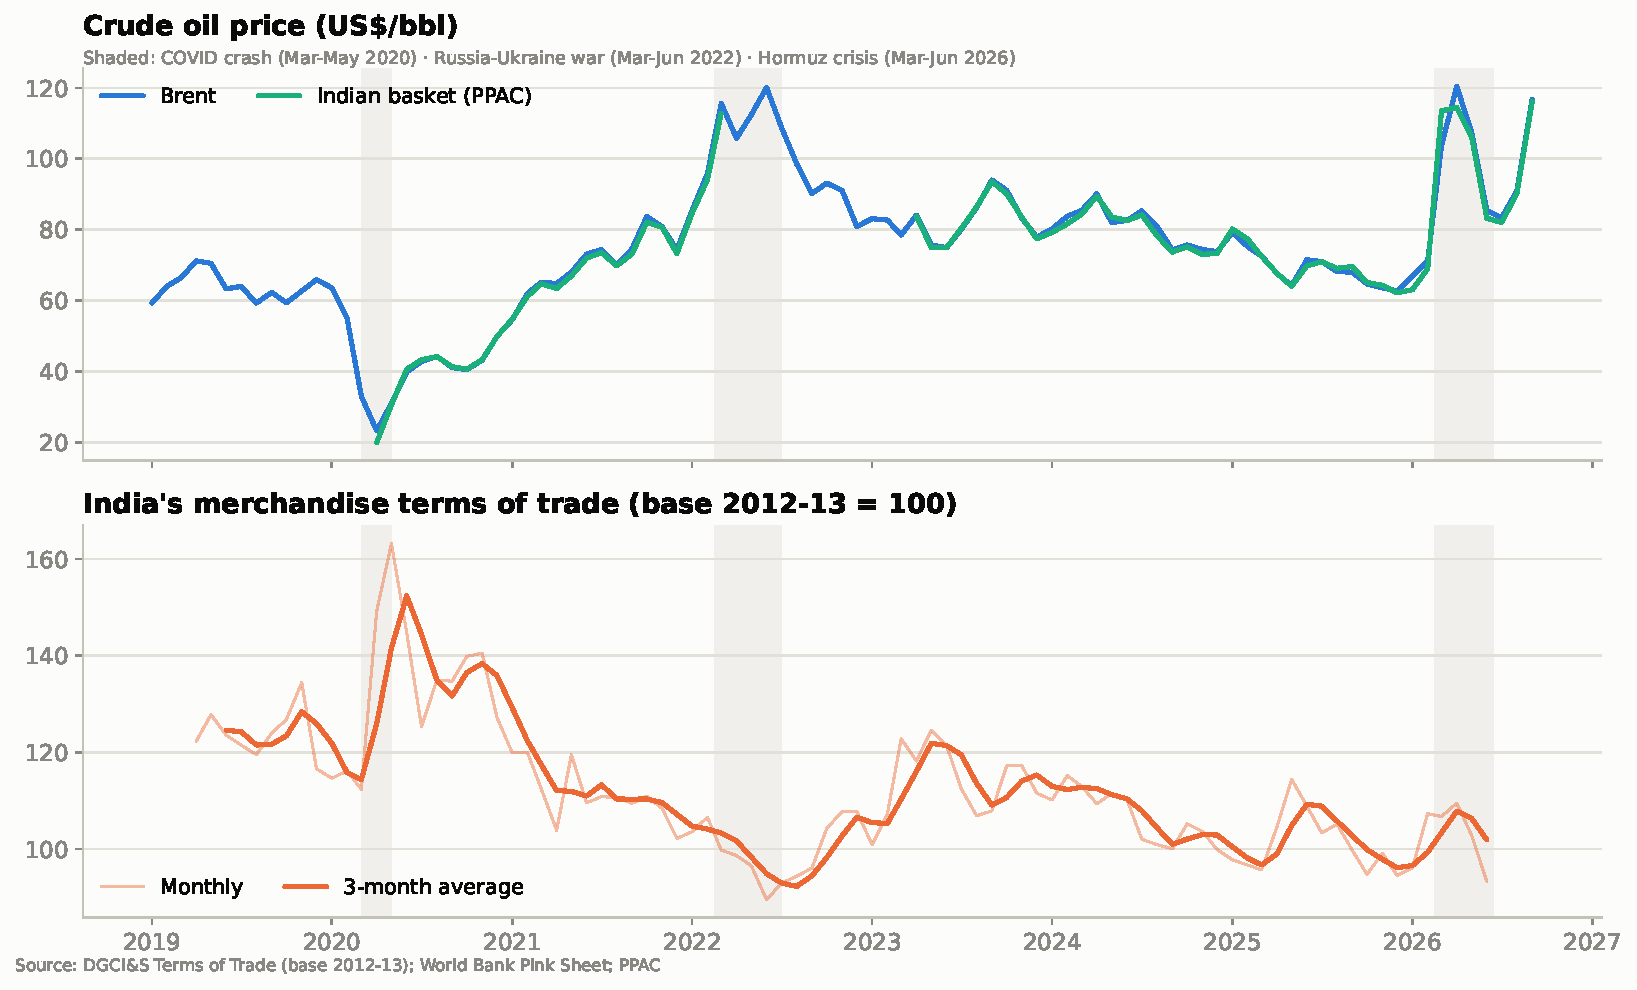
\includegraphics[height=0.58\textheight]{fig02_monthly_ntt_brent.pdf}
        \caption{Monthly merchandise ToT with 3-month moving average}
      \end{figure}
    \end{column}
    \begin{column}{0.45\textwidth}
      \textbf{2022 Russia-Ukraine:}
      \begin{itemize}
        \item Clear collapse: merchandise ToT fell $\sim$23.7\% (FY21$\to$FY23).
        \item Consistent with ARDL predictions.
      \end{itemize}
      \vspace{0.3cm}
      \textbf{2026 Hormuz Episode:}
      \begin{itemize}
        \item No clear collapse yet --- may reflect the refining hedge.
        \item Data provisional and noisy.
        \item Treated with ``honest uncertainty.''
      \end{itemize}
    \end{column}
  \end{columns}
\end{frame}

% ============================================================
\section{Policy Implications}
% ============================================================

% SLIDE 22
\begin{frame}{Policy Implications}
  \begin{table}[ht]
    \centering\small
    \begin{tabular}{>{\bfseries}p{3.5cm} p{10cm}}
      \toprule
      \textbf{Policy Area} & \textbf{Implication} \\
      \midrule
      Strategic Petroleum Reserves & Most ToT damage arrives in 2--3 months. SPR releases can smooth this high-impact short-run window. \\[4pt]
      Fuel-Tax Buffer & Rises and falls are symmetric $\Rightarrow$ counter-cyclical fuel taxes can smooth both spikes and slumps. \\[4pt]
      Refining Capacity & Maintaining competitive refining \& petrochemical exports acts as a \textbf{natural hedge}. \\[4pt]
      Energy Transition & Demand-driven commodity booms hurt too. Reducing fossil fuel dependence lowers the underlying $s_m$. \\
      \bottomrule
    \end{tabular}
  \end{table}
\end{frame}

% ============================================================
\section{Limitations}
% ============================================================

% SLIDE 23
\begin{frame}{Limitations and Caveats}
  \begin{itemize}
    \item \textbf{Unit value indices} combine price changes with product-mix and quality changes (not pure price indices).
    \item \textbf{Monthly sample} is relatively short (Apr 2019--Jun 2026, $\sim$87 months) $\Rightarrow$ wider uncertainty bands in local projections.
    \item \textbf{G\&S measure} includes services, which dilutes the pure oil-price effect.
    \vspace{0.3cm}
    \item \textbf{Mitigation strategies:}
    \begin{itemize}
      \item Used two independent ToT measures (G\&S and merchandise).
      \item Structural benchmark ($s_x - s_m$) as an independent cross-check.
      \item Identified shocks (Baumeister--Hamilton, K\"anzig) to address endogeneity.
      \item CUSUM stability tests confirm parameter constancy.
    \end{itemize}
  \end{itemize}
\end{frame}

% ============================================================
\section{Conclusion}
% ============================================================

% SLIDE 24
\begin{frame}{Summary of Findings}
  \begin{enumerate}
    \item \textbf{Short-Run Vulnerability (H1 $\checkmark$):} A 10\% real oil-price increase worsens India's ToT by $\approx 2.4\%$ in the short run.
    \vspace{0.2cm}
    \item \textbf{Timing:} Peak impact at $\sim$2 months; acts as a temporary shock with 31\% annual error correction.
    \vspace{0.2cm}
    \item \textbf{Symmetry (H2 $\times$):} Oil-price rises and falls have broadly symmetric effects.
    \vspace{0.2cm}
    \item \textbf{Supply $\approx$ Demand (H3 $\times$):} Demand-driven price increases hurt at least as much, due to broad commodity-price co-movement.
    \vspace{0.2cm}
    \item \textbf{The Headline:} India's exposure has \textbf{roughly halved} since the 1990s, explained by the growth of refined petroleum exports (RCA: $0.06 \to 4.37$) acting as an endogenous hedge.
  \end{enumerate}
\end{frame}

% ============================================================
\section{Literature Review}
% ============================================================

% SLIDE 25
\begin{frame}{Literature Review (I): ToT and Oil Shocks}
  \textbf{Terms-of-Trade Importance:}
  \begin{itemize}
    \item \textit{Harberger (1950); Laursen \& Metzler (1950):} ToT shocks affect real income, saving, and external balances (the ``Harberger--Laursen--Metzler'' effect).
    \item \textit{Obstfeld \& Rogoff (1995):} Extended to intertemporal open-economy models.
    \item \textit{Backus \& Crucini (2000):} Oil shocks as a primary driver of ToT fluctuations.
  \end{itemize}
  \vspace{0.3cm}
  \textbf{Oil Shocks and Macroeconomic Transmission:}
  \begin{itemize}
    \item \textit{Hamilton (1983, 2003):} Oil-price increases preceded most post-war U.S.\ recessions.
    \item \textit{Kilian (2009):} Not all oil shocks are alike --- supply disruptions, demand expansions, and speculation have different macro effects.
    \item \textit{Baumeister \& Hamilton (2019):} Structural decomposition with sign and elasticity restrictions.
    \item \textit{K\"anzig (2021):} OPEC supply-news instrument using high-frequency futures data.
  \end{itemize}
\end{frame}

% SLIDE 26
\begin{frame}{Literature Review (II): India and Research Gap}
  \textbf{The Indian Context:}
  \begin{itemize}
    \item Existing literature focuses on oil's effect on India's \textit{trade balance, inflation, exchange rate, and GDP growth}.
    \item \textit{Srinivasan \& Kalaivani (2013):} Oil-price shocks and current account in India.
    \item \textit{Rafiq et al.\ (2009):} Oil-price volatility and India's economic activity.
    \item Very little work models the ToT \textbf{directly} as the dependent variable.
  \end{itemize}
  \vspace{0.3cm}
  \textbf{Our Contribution:}
  \begin{itemize}
    \item First study to model India's NTT directly against oil prices using ARDL/NARDL.
    \item Estimates short-run and long-run elasticities; tests structural benchmark $(s_x - s_m)$.
    \item Links the decline in exposure to India's \textbf{acquired comparative advantage} in refining.
    \item Uses identified structural shocks (not just Brent price) as exogenous variation.
  \end{itemize}
\end{frame}

% ============================================================
\section{References}
% ============================================================

% SLIDE 27
\begin{frame}{References}
  \begin{thebibliography}{99}
    \setbeamertemplate{bibliography item}[text]
    \footnotesize
    \bibitem{backus2000} Backus, D.K.\ \& Crucini, M.J.\ (2000). Oil prices and the terms of trade. \textit{Journal of International Economics}, 50(1), 185--213.
    \bibitem{baumeister2019} Baumeister, C.\ \& Hamilton, J.D.\ (2019). Structural interpretation of vector autoregressions with incomplete identification. \textit{Journal of Monetary Economics}, 109, 48--65.
    \bibitem{hamilton1983} Hamilton, J.D.\ (1983). Oil and the macroeconomy since World War II. \textit{Journal of Political Economy}, 91(2), 228--248.
    \bibitem{harberger1950} Harberger, A.C.\ (1950). Currency depreciation, income, and the balance of trade. \textit{JPE}, 58(1), 47--60.
    \bibitem{kanzig2021} K\"anzig, D.R.\ (2021). The macroeconomic effects of oil supply news. \textit{American Economic Review}, 111(4), 1092--1125.
    \bibitem{kilian2009} Kilian, L.\ (2009). Not all oil price shocks are alike. \textit{American Economic Review}, 99(3), 1053--1069.
    \bibitem{laursen1950} Laursen, S.\ \& Metzler, L.A.\ (1950). Flexible exchange rates and the theory of employment. \textit{REStat}, 32(4), 281--299.
    \bibitem{obstfeld1995} Obstfeld, M.\ \& Rogoff, K.\ (1995). Exchange rate dynamics redux. \textit{JPE}, 103(3), 624--660.
  \end{thebibliography}
\end{frame}

% SLIDE 28
\begin{frame}{}
  \vfill
  \centering
  \Huge\bfseries Thank You!\\[0.5cm]
  \large Questions?
  \vfill
\end{frame}

\end{document}
